%\subsection{Программный комплекс ``Conver''}
\label{sec:Conver}

%Для построения описанных выше моделей использовался разработанный в ЦАГИ программный комплекс ``Conver''. 
%Его использование позволило многократно сократить время построения каждой модели. 

%\subsection{Описание комплекса}
Комплекс представляет собой многоуровневую среду для автоматизированного проектирования и оптимизации ЛА. Комплекс делится на 4 уровня по степени детализации:



\begin{figure}[ht]
\centering
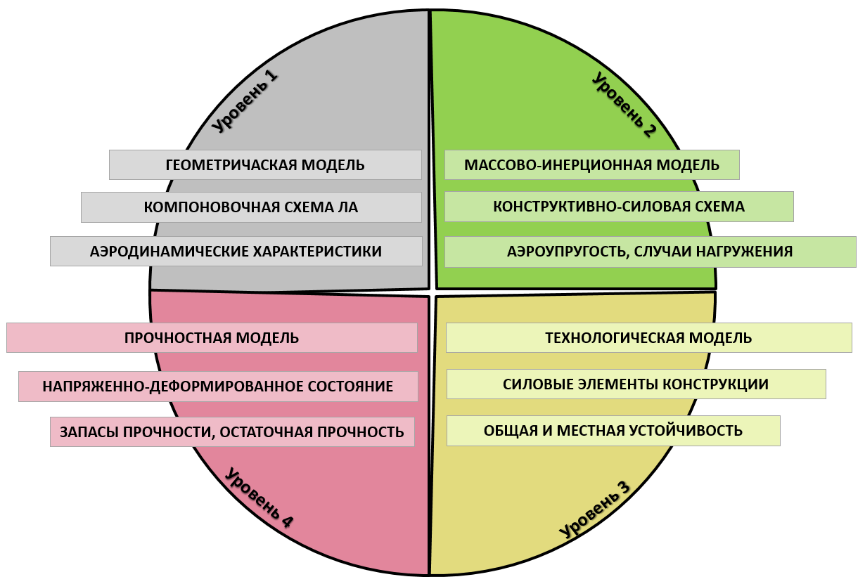
\includegraphics[width=0.6\textwidth]{ConverCircle} 
\caption{Принципиальная схема четырехуровневого проектирования}
\end{figure}



\begin{itemize}
\item Уровень 1: расчёт аэродинамических нагрузок и аэродинамических характеристик; 
\item Уровень 2: расчёт инерционных нагрузок, формирование случаев нагружения, решение задач статической и динамической аэроупругости, анализ веса конструкции планера;
\item Уровень 3: расчёт местной и общей устойчивости, анализ закритического состояния отдельных элементов конструкции, расчёт нелинейного НДС панелей гермокабины, расчет несущей способности элементов конструкции;
\item Уровень 4: расчёт общего НДС конструкции ЛА, определение запасов прочности, определение остаточной прочности, расчет длительной прочности.
\end{itemize}

Основные особенности программного комплекса:

\begin{enumerate}
\item Эффективное проведение параметрических исследований для различных конструкций планера, что позволяет минимизировать временные затраты и снизить трудоёмкость всего процесса;
\item Обеспечение более высокого качественного уровня параметрических исследований на начальной стадии проектирования за счёт автоматизированного создания полноразмерных моделей конструкции ЛА и автоматизации процесса анализа результатов исследований;
\item Оперативная оценка веса конструкций летательных аппаратов с учётом технологических ограничений при автоматическом использовании специализированных баз данных поправочных технологических коэффициентов.
\item Оперативность создания и изменения МКЭ-модели
\item Удобство взаимодействия программного комплекса с другими программами (см.Рис.\ref{fig:InterProgramScheme})
\end{enumerate}

Описанные выше особенности комплекса делают его удобным инструментом для задачи проектирования параметрической МКЭ-модели БПЛА. 

\begin{figure}
\centering
\def\svgwidth{0.8\textwidth}
%\input{figures/InterProgramScheme.pdf_tex}

\includegraphics[width=0.8\textwidth]{InterProgramScheme}
\caption{Схема взаимодействия комплекса ``Conver'' с другими программными продуктами}
\label{fig:InterProgramScheme}
\end{figure}


%\subsection{Внесенные изменения}

В ходе работы, для повышения степени автоматизации процесса был создан новый интерфейс  для первого уровня комплекса. 

\begin{figure}[h]
\centering
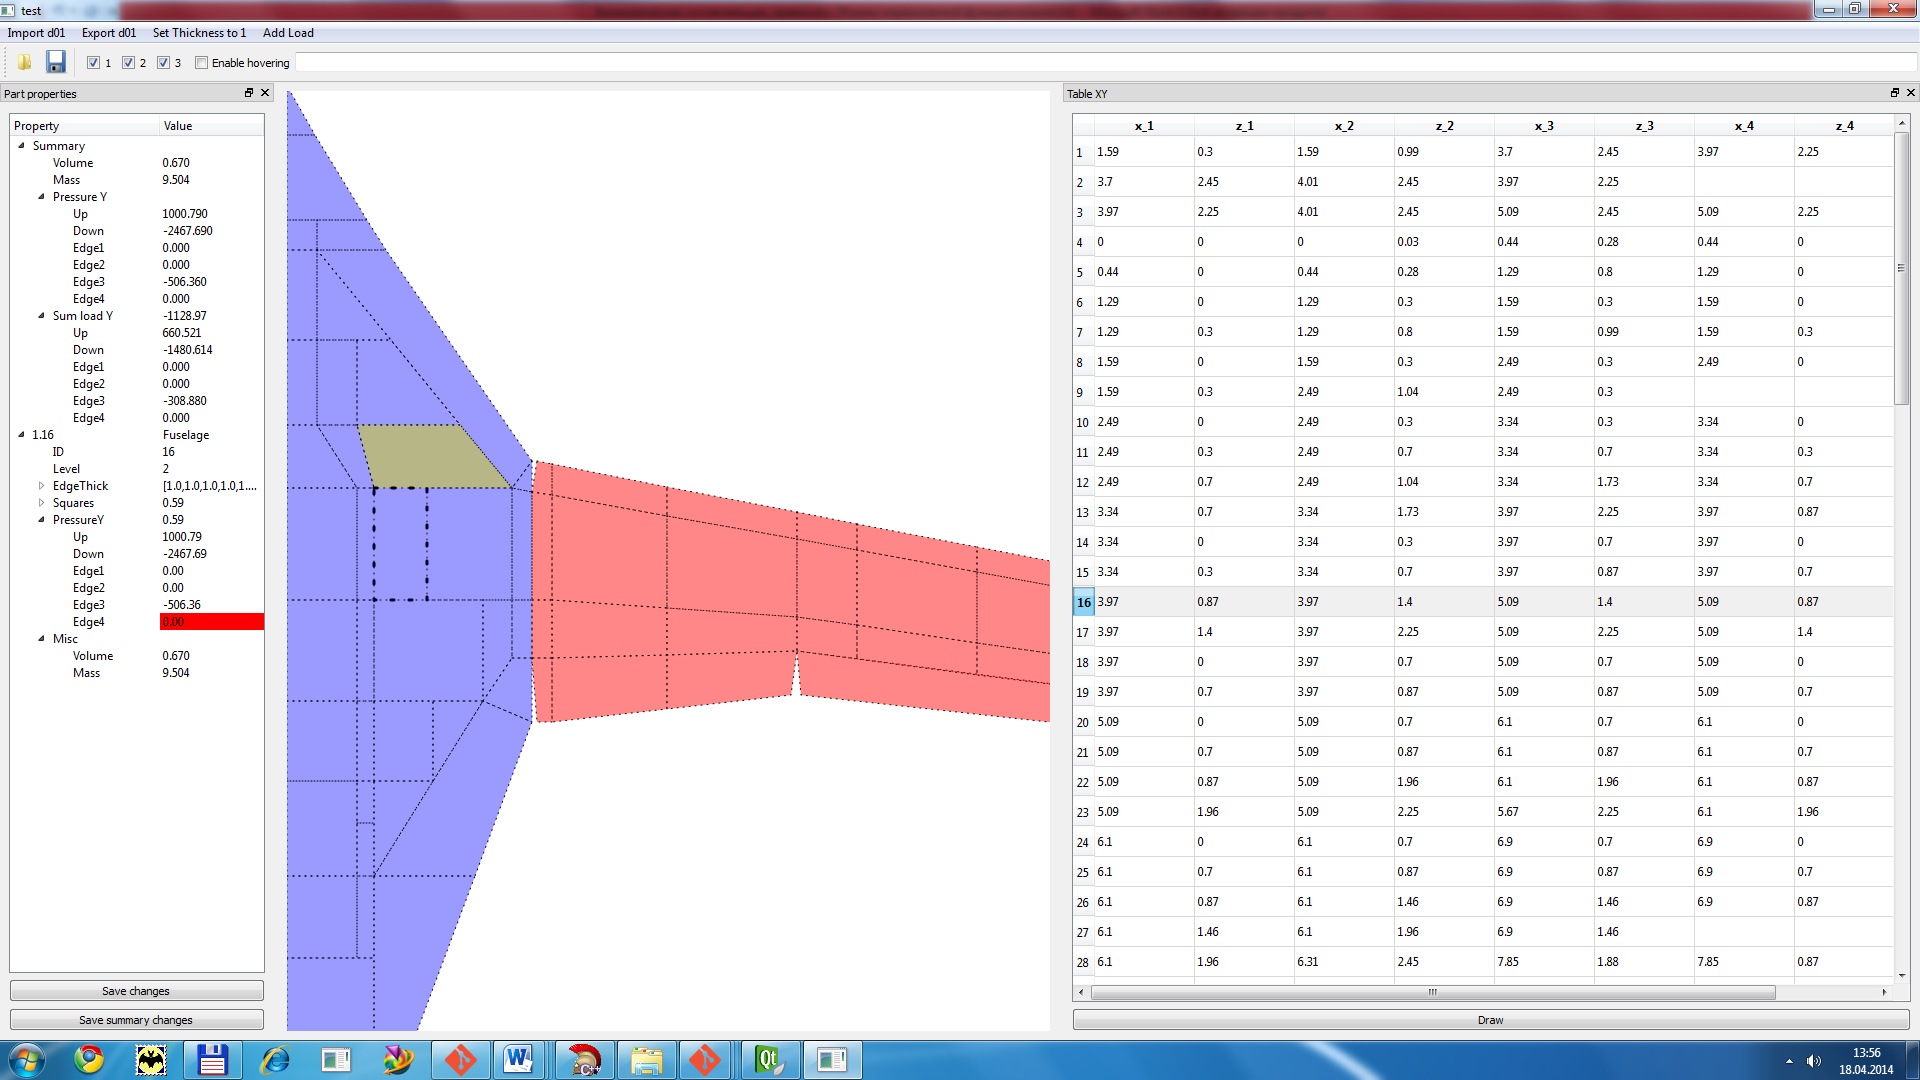
\includegraphics[width=0.8\textwidth]{ConverNewInterfaceOverview}
\caption{Новый интерфейс программного комплекса ``Conver''}
\label{fig:ConverNewInterfaceOverview}
\end{figure}


В новом интерфейсе были реализованы следующие изменения:

\begin{itemize}
	\item Полностью переработана система визуализации
	\begin{itemize}
		\item Добавлены инструменты масштаба и перемещения
		\item Добавлена двусторонняя связь между схемой и областями ввода данных
		\item Добавлена возможность отображения каждого этажа в 		схеме по отдельности
		\item Добавлено отображение ошибок во введенных данных
	\end{itemize}
	\item Переработана система ввода параметров отсеков
	\begin{itemize}
		\item Добавлены визуальные подсказки, предупреждающие ошибки в данных
		\item Добавлена возможность ввода параметров сразу для нескольких отсеков
	\end{itemize}
	\item Добавлена возможность ввода нагрузок непосредственно через задание сил, действующих на отсек
	\item Добавлена возможность просмотра данных, получаемых из других уровней комплекса:
	\begin{itemize}
		\item Оценочный расчет веса конструкции или выбранных отсеков
		\item Расчет объема выбранных отсеков
		\item Просмотр площадей стенок отсеков
	\end{itemize}
\end{itemize}

Рассмотрим, как изменилась работа с типовыми операциями, с которыми приходится сталкиваться пользователю. 


\subsection{Сравнение работы с типовыми операциями в старой и новой версии интерфейса}

\subsubsection{Изменение толщин в отсеке}

Задача: изменить толщину отсека в центроплане. 

\paragraph{Прежний подход:} 

\begin{itemize}
\item Найти номер отсека по схеме (Рис.\ref{fig:ConverListxzOld}) ($\sim1-3~\text{мин.}$)
\item Найти соответствующую ячейку в таблице толщин. ($\sim15~\text{сек.}$)
\item Изменить значение в ячейке. ($\sim5~\text{сек.}$)
\end{itemize}

Итого: $\sim3~\text{мин.}$

\begin{figure}[ht]
\centering
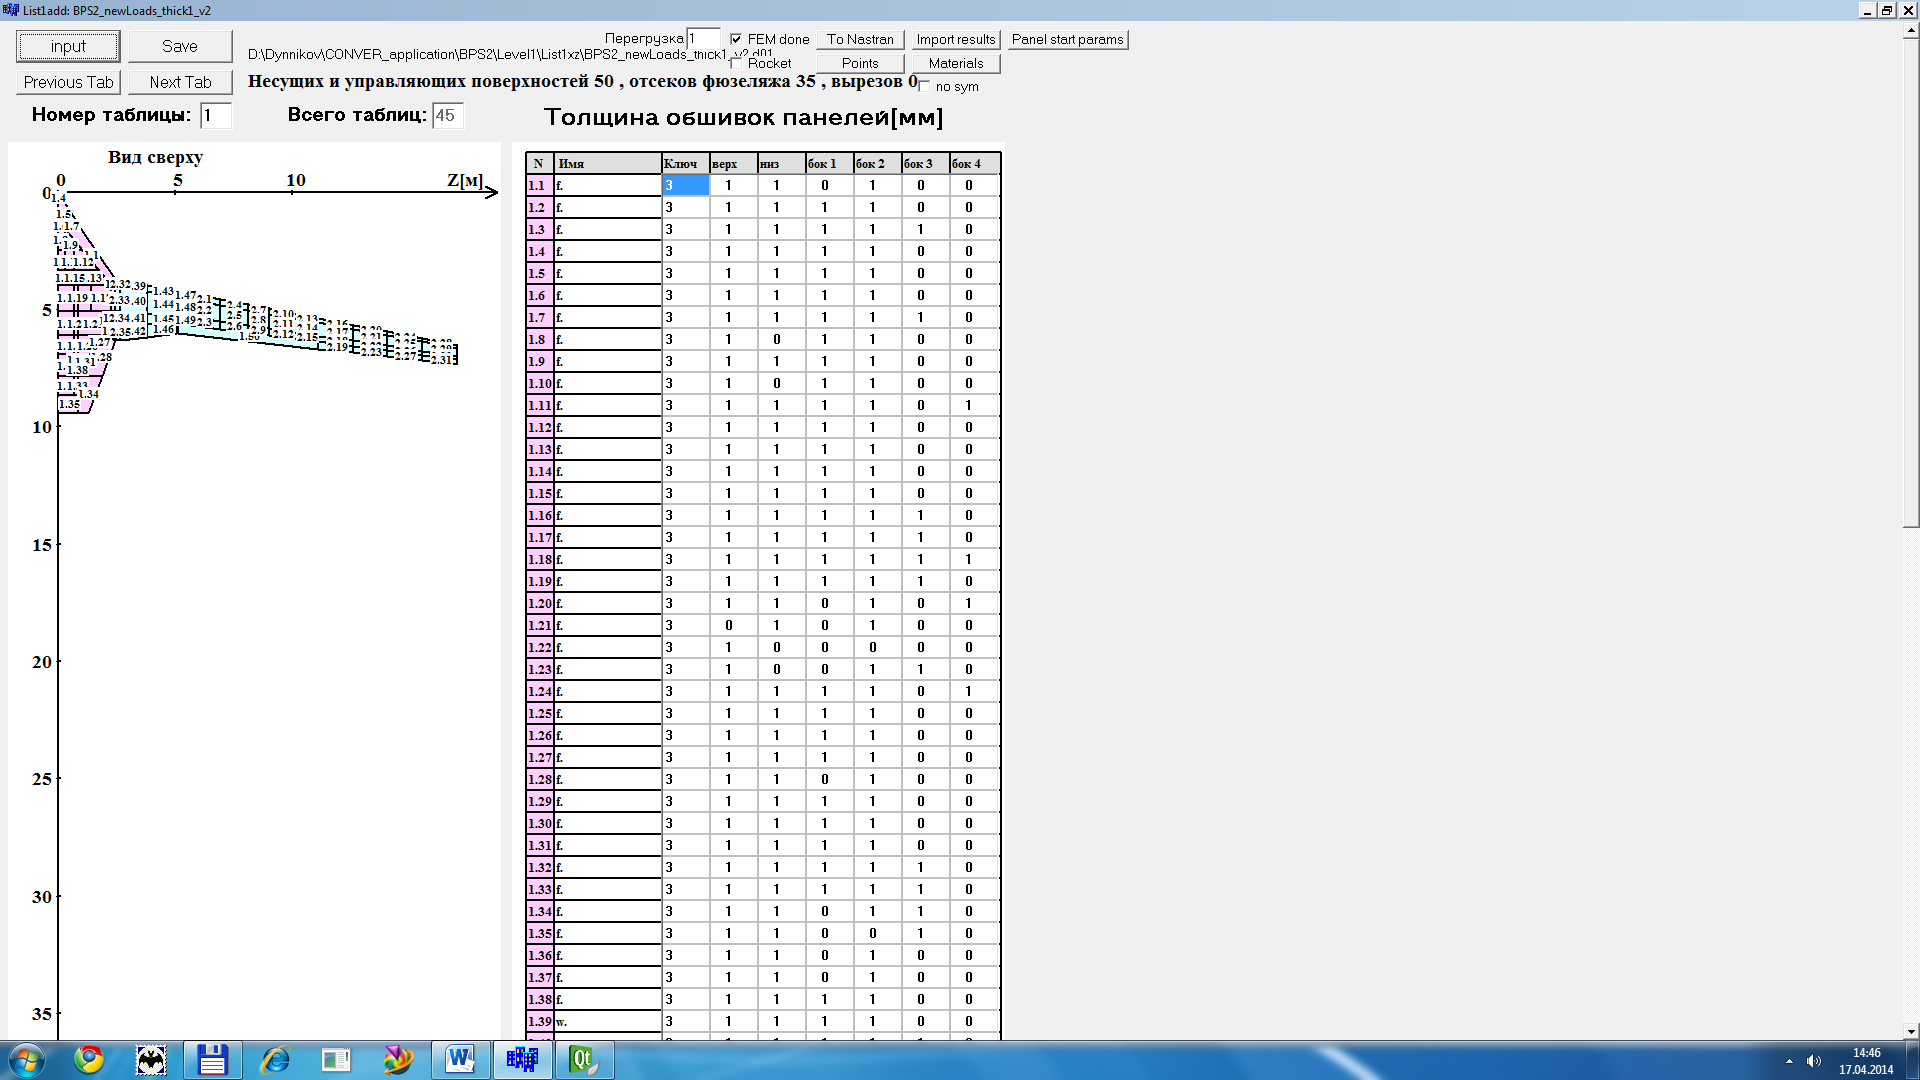
\includegraphics[width=0.8\textwidth]{ConverListxzOld}
\caption{Окно отображения отсеков в предыдущей версии интерфейса}
\label{fig:ConverListxzOld}
\end{figure}

\paragraph{Новый подход:}

\begin{itemize}
\item Кликнуть на нужный отсек на схеме (Рис.\ref{fig:ConverListxzOld}) ($\sim5~\text{сек.}$)
\item Изменить значение в ячейке толщины нужной стенки($\sim5~\text{сек.}$)
\end{itemize}

Итого: $\sim10~\text{сек.}$

\begin{figure}[ht]
\centering
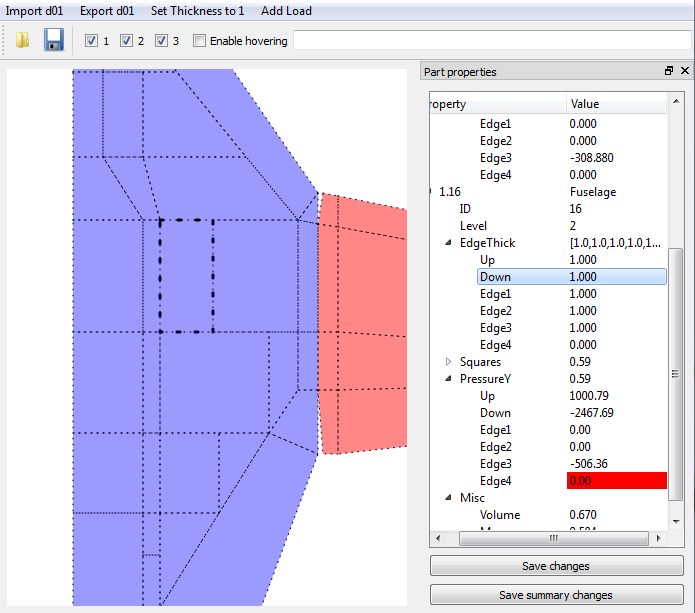
\includegraphics[width=0.8\textwidth]{ConverNewChangingThicks}
\caption{Окно отображения отсеков в новой версии интерфейса}
\label{ConverNewChangingThicks}
\end{figure}

\subsubsection{Нагружение отсека заданной силой}

Задача: по визуальному нахождению стенки нагрузить её заданной силой.

\paragraph{Прежний подход:}

\begin{itemize}
\item Найти по схеме (Рис.\ref{fig:ConverListxzOld}) отсеки, в которых может быть определена нужная стенка ($\sim5~\text{мин.}$)
\item Найти в таблице толщин, какой из выбранных отсеков имеет толщину этой стенки отличную от нуля($\sim3~\text{мин.}$)
\item Из 4 уровня программы найти площадь этой стенки($\sim3~\text{мин.}$)
\item По площади стенки найти давление, которое необходимо на неё приложить($\sim1~\text{мин.}$)
\item В таблице давлений найти нужную ячейку и ввести в неё полученную величину($\sim5~\text{мин.}$)
\end{itemize}

Итого: $\sim17~\text{мин.}$

\paragraph{Новый подход:}

\begin{itemize}
\item Кликнуть на один из отсеков, которому принадлежит эта стенка($\sim10~\text{сек.}$)
\item Если ячейка давления на нужную стенку выделена красным, выбрать другой отсек, в котором эта ячейка не выделена красным, то есть в которой эта стенка имеет ненулевую толщину($\sim1~\text{мин.}$)
\item Нажать кнопку ``Add load''  ($\sim10~\text{сек.}$)
\item В открывшемся окне (Рис.\ref{fig:ConverAddLoad}) ввести величину прикладываемой силы и выбрать стенки отсека, на которые должна быть распределена данная нагрузка. ($\sim30~\text{сек.}$) 
\item Нажать ``Add load'' ($\sim10~\text{сек.}$)

\end{itemize}

Итого: $\sim2~\text{мин.}$

\begin{figure}[ht]
\centering
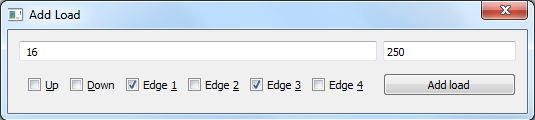
\includegraphics[width=0.5\textwidth]{ConverNewInterfaceAddLoad}
\caption{Окно добавления нагрузок в новой версии интерфейса}
\label{fig:ConverAddLoad}
\end{figure}